%\VignetteIndexEntry{CMA Manual}
%\VignetteKeywords{Classification}
%\VignetteDepends{CMA}
%\VignettePackage{CMA}

\documentclass[a4paper, 10pt]{article}

%%% packages

%\usepackage{german}
%\usepackage[german]{babel}
\usepackage[latin1]{inputenc}
\usepackage{amsfonts}
\usepackage{amssymb}
\usepackage{amsmath}
\usepackage{amsthm}
\usepackage{latexsym}
\usepackage{verbatim}
\usepackage{epsfig}
\usepackage{fleqn}
\usepackage{color}
\usepackage[colorlinks=true, linkcolor=blue, anchorcolor=blue,
											citecolor=blue, filecolor=blue, menucolor=blue, pagecolor=blue,
											urlcolor=blue]{hyperref}
\usepackage{mathrsfs}
\usepackage{eufrak}
\usepackage{graphicx}
\usepackage{multicol}
\usepackage{amsbsy}
\usepackage{bm}
\usepackage[nonamebreak,square]{natbib}
\usepackage[ruled]{algorithm2e}
%\setcitestyle{authoryear,aysep={},yysep={;},numbers}

%%% page layout

\parindent0pt
\parskip1ex
\oddsidemargin-0.5cm
\topmargin-.2cm
\textheight23cm
\textwidth13cm
\headsep0.5cm
%\usepackage{E:/R_Installation/share/texmf/Sweave}
\pagestyle{plain}

%%% Operators

\newcommand{\R}{{\mathbb R}}
\DeclareMathOperator*{\var}{var}
\DeclareMathOperator*{\cov}{cov}
\DeclareMathOperator*{\tr}{tr}
\DeclareMathOperator*{\diag}{diag}
\newcommand{\E}{\textbf{E}}
\DeclareMathOperator*{\p}{\textbf{P}}
\providecommand{\wt}[1]{\widetilde#1}
\providecommand{\wh}[1]{\widehat#1}
\providecommand{\norm}[1]{\lVert#1\rVert}
\providecommand{\sp}{\langle \cdot, \cdot \rangle}
\providecommand{\M}[1]{\mathbf#1}
%\providecommand{\B}[1]{\bm#1}
\providecommand{\mc}[1]{\mathcal#1}
\providecommand{\T}{\top}
\newcommand{\sign}{\operatorname{sign}}
\newcommand{\logit}{\operatorname{logit}}

\def\su{\sum_{i=1}^n}
\def\etall{\mbox{{\it et al., }}}
\def\etal{\mbox{{\it et al. }}}



\title{\large{\texttt{CMA}} package vignette}
\author{Martin Slawski \footnote{\url{Martin.Slawski@campus.lmu.de}}\\
        Anne-Laure Boulesteix \footnote{\url{http://www.slcmsr.net/boulesteix}}}

\usepackage{/home/mcarlson/arch/x86_64/R-2-7/share/texmf/Sweave}
\begin{document}
\date{\normalsize{Sylvia Lawry Centre, Hohenlindenerstr. 1, D-81677 Munich, Germany}}
\maketitle


\section{Statistical background}
\label{sec:0}
For the last few years, microarray-based class prediction has been a major
topic in statistics and machine learning. 
Traditional methods often yield unsatisfactory results or are 
even inapplicable in the $p \gg n$ setting.
Hence, microarray studies have stimulated the development of 
new approaches and motivated the adaptation of known traditional methods
to high-dimensional data.
 
Moreover, model selection and evaluation of prediction rules 
proves to be highly difficult in this situation for several reasons.
Firstly, the hazard of overfitting, which is common to all prediction problems,
is increased by high dimensionality. Secondly, the usual evaluation scheme based
on the splitting  into learning and test data sets often applies only partially in
the case of small samples.
Lastly, modern classification techniques rely on the proper choice of hyperparameters 
whose optimization is highly computer-intensive, especially in the case of
high-dimensional data.


\section{Class prediction based high-dimensional data with small samples}\label{sec:1}
\subsection{Settings}
The classification problem can be briefly outlined as follows:
\begin{itemize}
\item we have a predictor space $\mc{X}$, here $\mc{X} \subseteq \R^p$
\item we have a finite set of class labels $\mc{Y} = \{0,\ldots,K-1\}$,
      with $K$ denoting the total number of classes
\item $P(\bm{x},y)$ denotes the joint probability distribution on $\mc{X} \times \mc{Y}$
\item we are given a finite sample $S = \{(\bm{x}_1,y_1),\ldots,(\bm{x}_n,y_n) \}$
      of $n$ predictor-class pairs.
\end{itemize}

%%% correct
The task is to find a decision function
\begin{align*}
\begin{split}
\widehat{f}: \; \mc{X}\; \rightarrow \; & \mc{Y}  \\
\bm{x} \mapsto & \widehat{f}(\bm{x})
\end{split}
\end{align*}
(the $\widehat{\cdot}$ indicates estimation from the given sample $S$) 
such that the \emph{generalization error}
\begin{equation}\label{riskfunctional}
R[f] = \E_{P(\bm{x},y)}[L(f(\bm{x}), y)] = \int_{\mc{X} \times \mc{Y}}  L(y, f(\bm{x})) \; d P(\bm{x},y)
\end{equation}
is minimized.  
$L(\cdot, \cdot)$ is a suitable loss function, usually taken to
be the indicator loss ($1, \; \text{if} \; f(\bm{x}) \neq y$, $0, \text{otherwise}$).
%Other loss functions and performances measures are discussed extensively in
%section \ref{sec:2}.\\

\subsection{Estimation of prediction accuracy}

As we are only equipped with a finite sample $S$ and the underlying distribution
is unknown, approximations to (\ref{riskfunctional}) have to be found. Its
empirical counterpart
\begin{equation}\label{erisk}
R[f]_{\text{emp}} = n^{-1} \su L(y_i, f(\bm{x}_i))
\end{equation}
has a (usually large) negative bias for (\ref{riskfunctional}), thus model
selection based on (\ref{erisk}) leads to overfitting the sample $S$.\\
A first improvement involves a split of into parts $\mc{L}$ (learning sample),
$\mc{T}$ (test sample) with the intention to separate model selection and
-evaluation, by doing model selection only with $\mc{L}$ and evaluating the
resulting decision function $f(\cdot)$ only on $\mc{T}$.

For microarray data, the sample sizes $n$ is usually very small, leading to 
serious problems when estimating prediction accuracy 
and when constructing a prediction rule based on the available data, a problem which is also
related to model choice (see Section \ref{subsec:pred}). 

When splitting the original data into two approximately equally sized 
data sets (learning set and test set), the performance
of $f(\cdot)$ is strongly diminuished due to a further reduction of the sample
size and the evaluation is unreliable and highly variant. Hence, alternative
designs are needed.

In the package \texttt{CMA}, we pursue the following route for mitigating at least
the second consequence, by resampling and aggregating:
\begin{itemize}
\item Generate $B$ splits of $S = (\mc{L}_b, \mc{T}_b), b=1,\ldots,B$
      into learning- and test sample
\item Obtain $\widehat{f}_b$ from $\mc{L}_b, \; b=1,\ldots,B$
\item Setting  $\mc{I}_b = \{i: y_i \notin \mc{L}_b \}$, we use
      \begin{equation}\label{errorglobal}
      \wh{\varepsilon} = \frac{1}{B} \sum_{b=1}^B \frac{1}{|\mathcal{I}_b|}
                                     \sum_{i \in \mathcal{I}_b} I(y_i \neq \widehat{f}_b(\bm{x}_i))
      \end{equation}
      as estimator for (\ref{riskfunctional}).                                 
\end{itemize}
The strategy is to reduce the variance of the error estimator by averaging.\\
If $n$ is large, this procedure will not improve much on a simple splitting.\\
As splitting rules, the function \texttt{GenerateLearningsets} implements:
\begin{itemize}
\item \textbf{Leaving-one-out cross-validation} :\\
      $\mc{T}_b$ consists only of one observation, this is repeated
      for each observation in $S$, so that $B = n$.
\item $k$-\textbf{fold cross-validation} (\texttt{method = "CV", fold = , niter = }):\\
      $S$ is split into $k$ parts of equal size. For each iteration $b$,
      the $b$-th part is used as $\mc{T}_b$ and the union of the remaining
      parts as $\mc{L}_b$. Setting $\texttt{fold = n}$ 
      is equivalent to \texttt(method = "LOOCV"). 
      As the splitting is not uniquely determined for \texttt{fold} $< n$,
      the whole procedure can be repeated $\texttt{niter}$ times. 
\item Monte-Carlo-cross-validation (\texttt{method = "MCCV", fold=, ntrain=, niter= }):\\
      $B$=\texttt{niter} random learning samples of cardinality $\texttt{ntrain}$
      are generated.     
\item Bootstrap (\texttt{method = "bootstrap",  ntrain = , niter = }):\\
      $B$=\texttt{niter} bootstrap samples of cardinality $\texttt{ntrain}$ are 
      used as learning samples. 
\end{itemize}
Furhermore, \emph{stratified sampling} is possible by setting the
argument \texttt{strat = TRUE}. This implies, that for each $\mc{L}_b$, 
the proportion of the classes $\{0,\ldots,K-1 \}$ is the same as for 
the full $S$. This option is very useful (and sometimes even necessary)
in order to guarantee that each class is sufficiently often represented
in each $\mc{L}_b$, in particular if there are classes that are small in size.\\
Benefits and drawbacks of above splitting rules are discussed in 
\citet{BragaNeto} and \citet{Molinaro}.\\

\subsection{Constructing a prediction rule}\label{subsec:pred}
The second main issue is the construction of a appropriate prediction rule. 
In microarray data analysis, we
have to deal with the $n\ll p$ situation, i.e. the number of predictors
exceeds by far the number of observations. Some class prediction methods 
only work for the case $n \ll p$, e.g. linear or qudratic discriminant analysis
which are based on the inversion of a matrix of size $p\times p$ and rank $n-1$.
In the $n\ll p$ setting, the hazard of
overfitting is especially acute: perfect separation of the classes 
for a given sample based on a high number of predictors is always
possible. However, the resulting classification rule may generalize
poorly on independent test data.

There are basically three approaches to cope with the $n\ll p$ setting: 
\begin{enumerate}
\item variable selection using, e.g., univariate statistical tests
\item regularization or shrinkage methods, such as the Support Vector
      Machine (\citet{Boser1992}), $\ell_2$ or $\ell_1$ 
      penalized logistic regression (\citet{Zhu2004}; \citet{glmpath}) 
      or Boosting  (\citet{Friedman2001}; \citet{Buhlmann2003}) from
      which some also perform variable selection
\item dimension reduction or feature extraction. Most prominent is the 
      Partial Least Squares method (\citet{Boulesteixpls}). 
\end{enumerate}
Most classification methods depend on a vector of hyperparameters $\bm{\lambda}$
that have to be correctly chosen. Together with variable selection, this is part of the
model selection and has thus to be performed separately for each learning sample
$\mc{L}_b$ to avoid bias (\citet{modelselection}). An optimal vector of
hyperparameters $\bm{\lambda}^{\text{opt}}$ is determined by defining a discrete set of
values whose performance is then measured by cross-validation. This involves
a further splitting step, which is sometimes called 'inner loop' or 
'nested' cross-validation (\citet{Sta2005a}).
More precisely, each learning set $\mc{L}_b$ is divided into 
$l=1,\ldots,k$ parts such that the $l$-th part
forms the test sample for the $l$-th (inner) iteration. 
Analogously to (\ref{errorglobal}),
this procedure can be used to derive an error estimator for each value on the grid 
of candiate hyperparameter values. The optimal vector $\bm{\lambda}^{\text{opt}}$ 
is chosen to minimize this error criterion. Note that there are often several 
such minimizers. Furthermore, the 
minimizer found by this procedure can be relatively far away from the true minimizer,
depending on how fine the discrete grid has been chosen.\\
The choice of the inner cross-validation scheme is difficult.  With a high $k$, 
computation times soon become prohibitively high. With a low $k$, the size of 
$\mc{L}_{b_l}, \; l=1,\ldots,k$ is strongly reduced compared to the complete 
sample $S$, which may have an impact on the derived optimal parameter values.
Nevertheless, nested cross-validation is commonly used in this context 
 (\citet{review1}).\\

Considering the computational effort required for hyperparameter optimization and 
the small sample sizes, one may prefer class prediction methods 
that do not depend on many hyperparameters and/or behave robustly against changes
of the hyperparameter values.     

\section{Overview of CMA features}\label{sec:2}
In a nutshell, the package has the following features.
\begin{itemize}
\item It offers a uniform, user-friendly interface to a total of 21 classification
      methods (\ref{methodsoverview}), comprising classical approaches (such as 
	discriminant analysis)
      as well as more sophisticated methods, e.g. Support Vector Machines (SVM) or
      boosting techniques. User-friendliness means that the input formats are
      uniform among different methods, that the user may choose between
      three different input formats and that the output
      is highly self-explicable and informative.
\item Probability estimations for predicted observations are provided 
      by most of the classifiers, with only a few exceptions. This is more
      informative than only returning class labels and enables a more
      precise comparison of different classifiers.
\item It automatically generates learning samples as explained in
      \hyperref[sec:1]{section }{\ref{sec:1}}, including the generation of stratified samples.
\item Preliminary variable selection (if any) is performed for each iteration 
	separately based on one of the following ranking procedures, using the method 
	\texttt{GeneSelection}:
      \begin{itemize}
      \item ordinary two-sample t.test (\texttt{method = "t.test"})
      \item Welch modification of the t.test (\texttt{method = "welch.test"})
      \item Wilcoxon rank sum test (\texttt{method = "wilcox.test"})
      \item F test (\texttt{method = "f.test"}) when $K>2$
      \item Kruskal-Wallis test (\texttt{method = "kruskal.test"}) when $K>2$
      \item 'moderated' t and F test, respectively, \\
             using the package \texttt{limma}(\citet{limma}) (\texttt{method = "limma"})
      \item One-step Recursive Feature Elimination (\citet{rfe}) (\texttt{method = "rfe"})
      \item random forest variable importance measure (\texttt{method = "rf"})
      \item the Lasso (\texttt{method = "lasso"})
      \item the elastic net (\texttt{method = "elasticnet"}) 
      \item componentwise boosting (\texttt{method = "boosting"})                               
      \item the ad-hoc criterion used in \citet{golub1999}                                
      \end{itemize}                                
      For most methods, the implementation is very fast. The package 
     \texttt{CMA} uses own functions instead of the pre-defined
      \texttt{R} functions.
      Additionally, the multi-class case is fully supported, even if the chosen
      \texttt{method} is not defined for it. The workaround is realized by using
      either a pairwise or a one-vs-all scheme. 
\item Hyperparameter tuning is carried out using the scheme outlined in section 
      \hyperref[sec:1]{section }{\ref{sec:1}},
      for a \emph{fixed} (sub)set of variables. 
	It can be performed in a fully automatically
      manner using pre-defined grids. Alternatively, it can 
	be completely customized by the user. 
\item The method \texttt{classification} enables the user to combine gene selection,
      hyperparameter tuning and class prediction into one single step. But each step
	can also be performed separately.
\item Performance can be assessed using several performance measures
	which are commonly used in practice: 
      \begin{itemize}
      \item the misclassification rate                                         
      \item the sensitivity and specifity, for $K=2$
      \item the empirical area under the curve (AUC), for $K=2$, if the class 
	prediction method returns a probability,
      \item the Brier score
      \item the average probability of correct classification                                
      \end{itemize}                          
	Each performance measure can be 1) averaged for all predictions globally,
	2) averaged within each iteration first and then over all iterations or 
	3) averaged within each observation first and then over all observations.
      Based on the results, the function \texttt{obsinfo} can be used to
      identify observations that are frequenly misclassified (and are thus
      candidates for outliers).
\item Comparison of the performance of several classifiers can be performed
	using one or several of the above performance measures. This comparison 
	can be tabulated and visualized using the method \texttt{comparison}.
\item Most results can quickly be summarized and visualized using pre-defined convenience
      methods, for example:
      \begin{itemize}
      \item \texttt{plot,cloutput-method} produces a probability plot,             also known as 'voting plot'
      \item \texttt{plot,genesel-method} visualizes variable importance via a barplot
      \item \texttt{roc,cloutput-method} draws the empirical ROC curve
      \item \texttt{toplist,genesel-method} shows the most important variables
      \item \texttt{summary,evaloutput-method} Makes a summary out of
        iteration- or observationwise performance measures 
      \end{itemize}
\item The implementation is fully organized in \texttt{S4} classes, thus making
      the extension of \texttt{CMA} very easy. In particular, own classification
      methods can easily be integrated if they return a proper object of class
     \texttt{cloutput}.
\item The class prediction methods implemented in \texttt{CMA} are summarized in Table
\ref{tab:methods}.                       
\end{itemize}

\begin{table}
\begin{tabular}[h!]{llll} \label{methodsoverview}
%\hline 
\textbf{method name} &\texttt{CMA} \textbf{function name} & \textbf{Package} & \textbf{Reference} \\
\hline
Componentwise Boosting & \texttt{compBoostCMA} &  \texttt{CMA} & \citet{Buhlmann2003} \\
Diagonal Discriminant Analysis & \texttt{dldaCMA}      &  \texttt{CMA} & \citet{dabook} \\
Elastic Net & \texttt{ElasticNetCMA} & \texttt{glmpath} & \citet{elasticnet} \\
Fisher's Discriminant Analysis& \texttt{fdaCMA} &   \texttt{CMA}          & \citet{Ripley1996} \\
Flexible Discriminant Analysis & \texttt{flexdaCMA} & \texttt{mgcv}    &  \citet{Ripley1996} \\ 
Tree-based Boosting &\texttt{gbmCMA} & \texttt{gbm} &   \citet{Friedman2001} \\
$k$-nearest neighbours & \texttt{knnCMA} & \texttt{class}             &   \citet{Ripley1996} \\
Linear Discriminant Analysis ${\ast}$ & \texttt{ldaCMA}      &  \texttt{MASS} & \citet{dabook} \\
Lasso & \texttt{LassoCMA}      &  \texttt{glmpath} & \citet{glmpath} \\
Feed-Forward Neural Networks & \texttt{nnetCMA} & \texttt{nnet} & \citet{Ripley1996} \\
Probalistic nearest neighbours & \texttt{pknnCMA} & \texttt{CMA} & $-$ \\
Penalized Logistic Regression & \texttt{plrCMA} & \texttt{CMA} &
\citet{Zhu2004} \\
Partial Least Squares ${\star}$ + $\ast$ & \verb+pls_ldaCMA+ & \texttt{plsgenomics} &
\citet{Boulesteixpls} \\
$\star$ + logistic regression & \verb+pls_lrCMA+ & \texttt{plsgenomics} & \citet{Boulesteixpls} \\
$\star$ + Random Forest & \verb+pls_rfCMA+ & \texttt{plsgenomics} & \citet{Boulesteixpls} \\
Probabilistic Neural Networks & \texttt{pnnCMA} &  \texttt{CMA} &
\citet{specht} \\
Quadratic Discriminant Analysis ${\ast}$ & \texttt{qdaCMA}      &  \texttt{MASS} & \citet{dabook} \\ 
Random Forest &\texttt{rfCMA} & \texttt{randomForest} &   \citet{Breiman2001} \\
PAM & \texttt{scdaCMA} & \texttt{CMA} & \citet{Tibshirani2002}   \\
Shrinkage Discriminant Analysis & \texttt{shrinkldaCMA} & \texttt{CMA} &  $-$ \\
Support Vector Machine & \texttt{svmCMA} &  \texttt{e1071} &
\citet{ScholkopfSmola2002} \\
\hline
\end{tabular}
\label{tab:methods}
\end{table}


\section{Comparison with existing packages}\label{sec:3}
The idea of an interace for the integration of classification methods for microarray
data is not new and we here argue why \texttt{CMA} can be a significant
improvement with respect to the following aspects: standardized and reproducible
analysis, neutral comparisons of existing methods, comfortable use.

The \texttt{CMA} package shows similarities to the \texttt{Bioconductor} 
package \texttt{MLInterfaces} standing for 'An interace to various machine 
learning methods' (\citet{Carey2007}), see  also the \text{Bioconductor} 
textbook  for a presentation of an older version. 

Contrary to \texttt{CMA}, \texttt{MLInterfaces} also offers access to popular 'unsupervised learning'
methods such as clustering, independent component analysis etc. that can
be beneficial for exploratory analyses as well as for revealing classes in
a preparatory step preceding supervised classification.
The package architecture is very similar the \texttt{CMA} structure in
the sense that wrapper functions are used to call classification methods from
other packages.

Up to now, \texttt{CMA} includes more predefined features than \texttt{MLInterfaces} 
as far as variable selection, hyperparameter tuning,
classifier evaluation and comparison are concerned. 
While the method \texttt{xval} is flexible for experienced users, it
provides only LOOCV or 'leave-one-group out' as predefined options.
As this package adresses also unexperienced users, we decided to include
the most common validation schemes in a standardized manner. As consequence,
we additionally hope to increase reproducibility of results which is a major
concern in statistics in general and for microarray data analysis in particular. 

In the current version, variable selection can also be carried separately for each different
learning set, but this seems not to be a standard procedure. In the examples
presented in the book mentionned above, variable selection is only performed once
using the \emph{complete} sample $S$ although this procedure is widely known 
to yield optimistically biased results (\citet{Amb2002}).

Moreover, hyperparameter tuning is completely missing in \texttt{MLInterfaces}. 
In our opinion, this makes the 
objective comparison of different class prediction methods difficult. 
If tuning is ignored, simpler methods without (or with few) tuning parameters
tend to perform seemingly better than more complex algorithms.

We 'borrowed' from \texttt{MLInterface} 
some ideas regarding the selection of
classification methods (\hyperref[sec:2]{section }{\ref{sec:2}}) 
and some functionalities such as the variable
importance plot, or the \texttt{Planarplot}. 
%For the sake of fairness of comparison, it
%has to be stated that our thorough test was unfortunately performed
%at a time where (according to the authors) \texttt{MLInterfaces} 
%is in a phase of new developments.

We would also like to mention the package \texttt{e1071} (\citet{e1071pack})
whose \texttt{tune} function served as the basic idea for the \texttt{CMA}
tuning functionalities.\\

The package \texttt{MCRestimate} (\citet{MCRestimate}) 
emphasizes very similar aspects as \texttt{CMA}, 
focussing on the estimation of misclassification rates and cross-validation for model 
selection and evaluation. It is (to our knowledge) the only \texttt{Biconductor}
package that supports hyperparameter tuning, but obviously referring to the
function \texttt{e1071:::tune}. Compared to \texttt{CMA}, it is a bit less comprehensive, in particular with respect
to variable selection. Moreover, the package structure is, to our opinion, less
stringent than that of CMA, mainly because it lacks a class structure (neither \texttt{S3}
nor \texttt{S4} is used).  

\section{Example 1: Focussing on one method}\label{sec:ex1}
The following two sections demonstrate the usual workflow when using
\texttt{CMA} and its essential features, methods and objects.
While this section focusses on optimizing and evaluating one method, the
following section is devoted to classifier comparison.

We use the famous leukaemia dataset of \citet{golub1999} as a data example. 
The sample consists of 38 observations in total, from which 27
belong to class 0 (acute lymphoblastic leukemia)  and 11 to class 1 (acute myeloid leukemia).
We start by loading and the dataset and extracting gene expression and class
labels, respectively.
\begin{Schunk}
\begin{Sinput}
> data(golub)
> golubY <- golub[, 1]
> golubX <- as.matrix(golub[, -1])
\end{Sinput}
\end{Schunk}

Following the approach described in \hyperref[sec:1]{section }{\ref{sec:1}}, we generate several learning samples
by different splitting rules, taking into account that each of them has advantages
and disadvantages.
Learning samples are generated by the function \texttt{GenerateLearningsets}, 
which returns an object of class \texttt{learningsets}:

\begin{Schunk}
\begin{Sinput}
> loodat <- GenerateLearningsets(y = golubY, method = "LOOCV")
> class(loodat)
> getSlots(class(loodat))
> show(loodat)
\end{Sinput}
\end{Schunk}

For five-fold cross-validation, we use the following commands:

\begin{Schunk}
\begin{Sinput}
> set.seed(321)
> fiveCVdat <- GenerateLearningsets(y = golubY, method = "CV", 
+     fold = 5, strat = TRUE)
\end{Sinput}
\end{Schunk}

Note that stratified learning sets are generated by setting the argument 
\texttt{strat = TRUE}. The random seed should be set for reproducibility. 
We can proceed analogously for Monte-Carlo cross-validation and bootstrap:

\begin{Schunk}
\begin{Sinput}
> set.seed(456)
> MCCVdat <- GenerateLearningsets(y = golubY, method = "MCCV", 
+     niter = 3, ntrain = floor(2/3 * length(golubY)), strat = TRUE)
> set.seed(651)
> bootdat <- GenerateLearningsets(y = golubY, method = "bootstrap", 
+     niter = 3, strat = TRUE)
\end{Sinput}
\end{Schunk}

In this example, we choose the Support Vector Machine with linear
kernel as classification method. Variable selection is not strictly necessary, 
but is has empirically been shown that the performance of the SVM method 
can significantly be improved when noise features are removed (\citet{Has2001}). 
For simplicity, we choose the distribution free
Wilcoxon-Test to rank the variables, separately for each learning sample :

\begin{Schunk}
\begin{Sinput}
> varsel_fiveCV <- GeneSelection(X = golubX, y = golubY, learningsets = fiveCVdat, 
+     method = "wilcox.test")
> varsel_MCCV <- GeneSelection(X = golubX, y = golubY, learningsets = MCCVdat, 
+     method = "wilcox.test")
> varsel_boot <- GeneSelection(X = golubX, y = golubY, learningsets = bootdat, 
+     method = "wilcox.test")
\end{Sinput}
\end{Schunk}

Now let us have a closer look at \verb+varsel_fiveCV+. The \texttt{toplist}
methods provides easy access to the top-ranked variables:

\begin{Schunk}
\begin{Sinput}
> show(varsel_fiveCV)
> toplist(varsel_fiveCV, iter = 1)
> seliter <- numeric()
> for (i in 1:5) seliter <- c(seliter, toplist(varsel_fiveCV, iter = i, 
+     top = 10, show = FALSE)$index)
> sort(table(seliter), dec = TRUE)
\end{Sinput}
\end{Schunk}

We see that no variable is among the top 10 in every learning sample; the highest
frequency is 4 out of 5.

The next step is hyperparameter tuning. It is well-known that the SVM
needs much tuning (\citet{Sta2005a}) and that its performance can decrease 
drastically without tuning. For simplicity, we use a linear kernel, thus avoiding the tuning of 
kernel parameters. The choice of the parameter $C$ in the primal objective
of the SVM
\begin{equation*}
P(\bm{w}) = \norm{\bm{w}}^2 + C \su \xi_i, \; C > 0
\end{equation*}
has still to be done. $\bm{w}$ denotes the weight vector of the maximum margin hyperplane,
while the $\{ \xi_i \}_{i=1}^n$ quantify the amount of violation of this
hyperplane by the learning sample. Increasing $C$ 
penalizes violations more severely, forcing the hyperplane to separate the
learning sample (and thus probably producing overfitting).\\
In order to find an appropriate value for $C$ (which corresponds to the argument
\texttt{cost} in \texttt{e1071:::svm}), we take the best 100 genes from the
previous variable ranking step. As hyperparameter tuning is very time-intensive, 
we use the five-fold CV procedure only
in this demonstrating example. The resulting best 
 value for \texttt{cost} will then also be used for the other other CV procedures. 
In this example, we consider five candidate values: 0.1,1,10,100,200.
Due to the nested cross-validation procedure, the SVM is trained 
$3 \times 5 \times 5 = 75$ times (!) in the following example. Three is to
the number of inner cross-validation folds, the first five is the number of candidate values
and the second five is the number of outer cross-validation folds.

\begin{Schunk}
\begin{Sinput}
> set.seed(351)
> tuningstep <- CMA:::tune(X = golubX, y = golubY, learningsets = fiveCVdat, 
+     genesel = varsel_fiveCV, nbgene = 100, classifier = svmCMA, 
+     grids = list(cost = c(0.1, 1, 10, 100, 200)))
\end{Sinput}
\end{Schunk}



\begin{Schunk}
\begin{Sinput}
> show(tuningstep)
> unlist(best(tuningstep))
\end{Sinput}
\end{Schunk}

It is evident that the results are rather unstable. In order to decide for
a suitable for the hyperparameter, we additionally visualize the results : 


\begin{Schunk}
\begin{Sinput}
> par(mfrow = c(2, 2))
> for (i in 1:4) plot(tuningstep, iter = i, main = paste("iteration", 
+     i))
\end{Sinput}
\end{Schunk}

Although it remains unclear which value is actually best, we take \texttt{cost
  = 100} because this never produced bad results.\\
We can now  turn the attention to class prediction:

\begin{Schunk}
\begin{Sinput}
> class_fiveCV <- classification(X = golubX, y = golubY, learningsets = fiveCVdat, 
+     genesel = varsel_fiveCV, nbgene = 100, classifier = svmCMA, 
+     cost = 100)
> class_MCCV <- classification(X = golubX, y = golubY, learningsets = MCCVdat, 
+     genesel = varsel_MCCV, nbgene = 100, classifier = svmCMA, 
+     cost = 100)
> class_boot <- classification(X = golubX, y = golubY, learningsets = bootdat, 
+     genesel = varsel_boot, nbgene = 100, classifier = svmCMA, 
+     cost = 100)
\end{Sinput}
\end{Schunk}

The results of \texttt{classification} are lists where each element is an
object of class \texttt{cloutput}, generated for each learning sample. For
visualization purpose, we use the \texttt{join} function to combine the single
list elements into 'big' objects. We first put the results from the
four splitting schemes into one list and then use \texttt{lapply()}:

\begin{Schunk}
\begin{Sinput}
> resultlist <- list(class_fiveCV, class_MCCV, class_boot)
> result <- lapply(resultlist, join)
\end{Sinput}
\end{Schunk}

The probability (or voting) plot is one of the most popular visualizatio method 
in microarray-based classification:

\begin{Schunk}
\begin{Sinput}
> schemes <- c("five-fold CV", "MCCV", "bootstrap")
> par(mfrow = c(3, 1))
> for (i in seq(along = result)) plot(result[[i]], main = schemes[i])
\end{Sinput}
\end{Schunk}

\texttt{ftable} applied to objects of class \texttt{cloutput} yields 
confusion matrices:

\begin{Schunk}
\begin{Sinput}
> invisible(lapply(result, ftable))
\end{Sinput}
\end{Schunk}
\texttt{roc} draws simple ROC cuves:

\begin{Schunk}
\begin{Sinput}
> par(mfrow = c(2, 2))
> for (i in seq(along = result)) roc(result[[i]])
\end{Sinput}
\end{Schunk}

We can now \texttt{join} again to aggregate over the different
splitting rules:

\begin{Schunk}
\begin{Sinput}
> totalresult <- join(result)
> ftable(totalresult)
\end{Sinput}
\end{Schunk}

Confusion matrices implicity quantify performance via
misclasification. For more advanced performance evaluation,
one can use \texttt{evaluation}. Note that the input has
to be a list (and not an object of class \texttt{cloutput}).
For the Monte-Carlo cross-validation scheme, we have:

\begin{Schunk}
\begin{Sinput}
> av_MCCV <- evaluation(class_MCCV, measure = "average probability")
> show(av_MCCV)
> boxplot(av_MCCV)
> summary(av_MCCV)
\end{Sinput}
\end{Schunk}

\texttt{measure = "average probability"} stands for the average predicted
probability for the correct class, or formally:

\begin{equation*}
\sum_{b=1}^B \sum_{i \in \mc{L}_b}  \sum_{k=0}^{K-1} I(y_i = k) \widehat{p}(y_i = k | \bm{x}_i), 
\end{equation*}
with $\widehat{p}(k|\bm{x})$ denoting the condtional predicted probability for class $k$,
given $\bm{x}$.\\
\\ 
By default, the evalution scheme is iterationwise, but it can also be done
observationwise :

\begin{Schunk}
\begin{Sinput}
> av_obs_MCCV <- evaluation(class_MCCV, measure = "average probability", 
+     scheme = "obs")
> show(av_obs_MCCV)
\end{Sinput}
\end{Schunk}

One might also wonder which observations are misclassified very often. To find
it out, one can use:

\begin{Schunk}
\begin{Sinput}
> obsinfo(av_obs_MCCV, threshold = 0.6)
\end{Sinput}
\end{Schunk}

\section{Example 2: classifier comparison}\label{sec:ex2}

\texttt{CMA} implements a complete bundle of methods based on the principle of
discriminant analysis. Here, we compare six of them:
diagonal-, linear- and quadratic discrimininant analysis, discriminant
analysis by Fisher, shrunken centroids discriminant analyis (also known
as PAM) and Partial Least Squares followed by linear discriminant analysis, 
, applied to the small blue round cell tumour dataset of \citet{Khan2001}
which comprises 65 samples from four tumour classes.\\ 
From a theoretical point of view, linear-, quadratic- and Fisher's discriminant
analysis are apriori inferior due to the fact that they do not work in the
$p \gg n$ without variable selection. Shruken centroids discriminant analysis
is assumed to work better than the simple diagonal discriminant analysis because
it can 'shrink-out' noise variables. Partial Least Squares is also expected to
work well.\\
But let as see how this looks in pratice. As data basis, we will use
(stratified) five-fold cross-validation, repeated ten times in order to
achive more stable results. 


 
\begin{Schunk}
\begin{Sinput}
> data(khan)
> khanY <- khan[, 1]
> khanX <- as.matrix(khan[, -1])
> set.seed(27611)
> fiveCV5iter <- GenerateLearningsets(y = khanY, method = "CV", 
+     fold = 5, niter = 5, strat = TRUE)
\end{Sinput}
\end{Schunk}

Contrary to the step-by-step procedure in the previous example, we will here always use
the flexible method \texttt{classification}. We start with diagonal
discriminant analysis which neither needs variable selection nor tuning. 


\begin{Schunk}
\begin{Sinput}
> class_dlda <- classification(X = khanX, y = khanY, learningsets = fiveCV5iter, 
+     classifier = dldaCMA)
\end{Sinput}
\end{Schunk}

We now rank the variables (genes) according to the t statistic as basis for
variable selection necessary for linear-, quadratic- and Fisher's linear discriminant
analysis:

\begin{Schunk}
\begin{Sinput}
> genesel_da <- GeneSelection(X = khanX, y = khanY, learningsets = fiveCV5iter, 
+     method = "t.test", scheme = "one-vs-all")
\end{Sinput}
\end{Schunk}

For the class prediction that follows, we pass the generated learning sets,
the gene rankings (\verb+genesel_da+) to \texttt{classification}. The
number of genes that are retained is specified by the argument \texttt{nbgene}.

\begin{Schunk}
\begin{Sinput}
> class_lda <- classification(X = khanX, y = khanY, learningsets = fiveCV5iter, 
+     classifier = ldaCMA, genesel = genesel_da, nbgene = 10)
> class_fda <- classification(X = khanX, y = khanY, learningsets = fiveCV5iter, 
+     classifier = fdaCMA, genesel = genesel_da, nbgene = 10, comp = 2)
> class_qda <- classification(X = khanX, y = khanY, learningsets = fiveCV5iter, 
+     classifier = qdaCMA, genesel = genesel_da, nbgene = 1)
\end{Sinput}
\end{Schunk}

Shrunken centroids discriminant analysis does not do variable selection, but
hyperparameter tuning for the shinkage intensity. We here use the pre-specified
grid by setting \texttt{tuninglist} to an empty list. 

\begin{Schunk}
\begin{Sinput}
> set.seed(876)
> class_scda <- classification(X = khanX, y = khanY, learningsets = fiveCV5iter, 
+     classifier = scdaCMA, tuninglist = list(grids = list()))
\end{Sinput}
\end{Schunk}
                             
At last, we use partial least squares (with two components, which is the default).

\begin{Schunk}
\begin{Sinput}
> class_plsda <- classification(X = khanX, y = khanY, learningsets = fiveCV5iter, 
+     classifier = pls_ldaCMA)
\end{Sinput}
\end{Schunk}

A comparison can be performed very quickly, needing only a very few lines. The method
\texttt{comparison} does the whole job: 

\begin{Schunk}
\begin{Sinput}
> dalike <- list(class_dlda, class_lda, class_fda, class_qda, class_scda, 
+     class_plsda)
> par(mfrow = c(3, 1))
> comparison <- compare(dalike, plot = TRUE, measure = c("misclassification", 
+     "brier score", "average probability"))
> print(comparison)
\end{Sinput}
\begin{Soutput}
        misclassification brier.score average.probability
DLDA           0.06433566  0.12460774           0.9364418
LDA            0.07244755  0.14352016           0.9278874
FDA            0.15664336  0.70803592           0.2717210
QDA            0.14713287  0.26636674           0.8505199
scDA           0.02377622  0.04316251           0.9710716
pls_lda        0.06321678  0.08706237           0.8917140
\end{Soutput}
\end{Schunk}
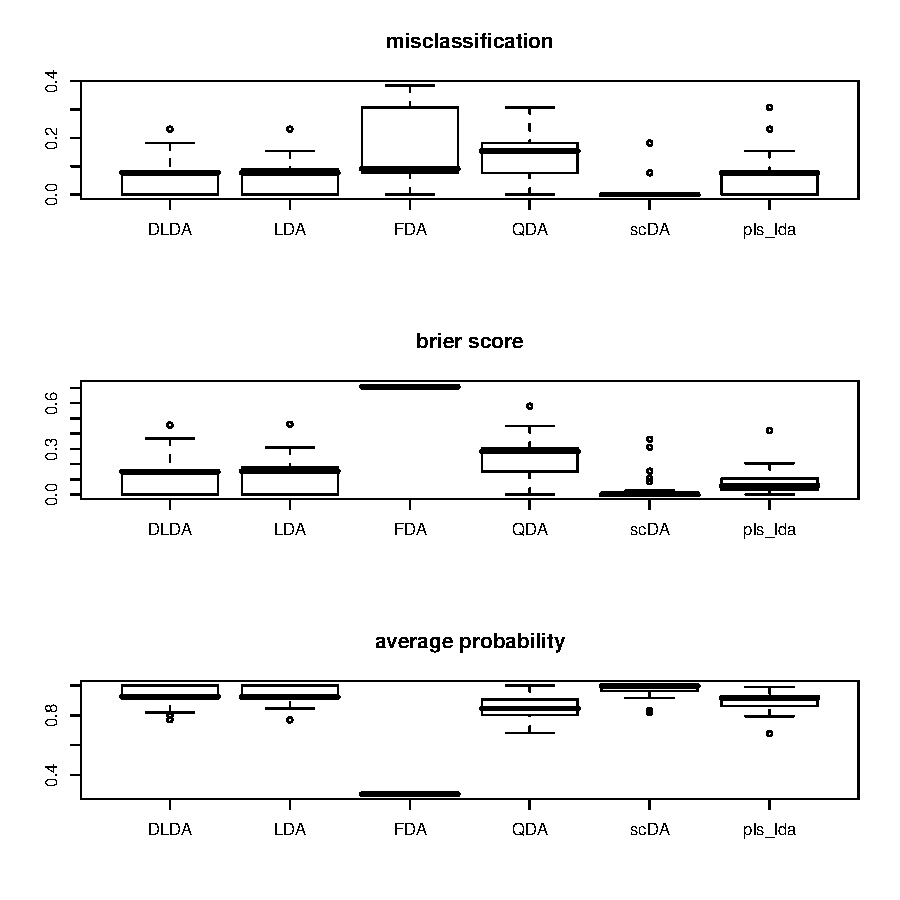
\includegraphics{CMA_annelaure-026}









\bibliographystyle{plainnat}
\bibliography{classification}

\end{document}











































































































     

       
        
